\section{Exemple d'application à un cas urbain}

Après avoir utilisé le cas-test Beaune pour tester plusieurs aspects de l'algorithme d'estimation, nous travaillons ici dans un cadre différent, qui est celui du milieu urbain. Plusieurs nouveaux facteurs d'incertitude sont ainsi introduits, et le but de ce paragraphe est d'examiner les résultats de l'AMIS dans un contexte à forte complexité.\\

\subsection{Présentation du cas-test}

Nous considérons désormais un cas-test en milieu urbain caractérisé par la présence d'obstacles multiples et de géométries variées sur le domaine (bâtiments). Pour cela, on utilise une reconstitution du quartier parisien de l'Opéra (figure \ref{fig_opera_config}), qui comme pour le cas-test Beaune, a initialement été utilisé pour la validation de RetroSPRAY.\\

\begin{figure}[h!]
	\centering
	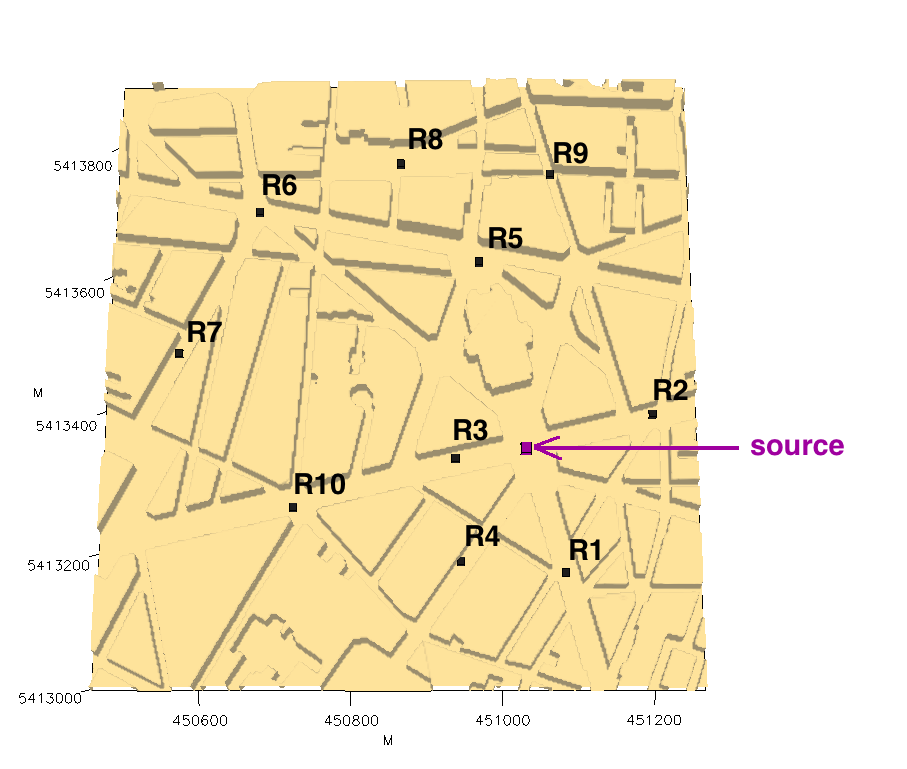
\includegraphics[width=0.6\textwidth]{opera_config_domaine.png}
	\caption{Illustration du milieu bâti, du réseau de capteurs (en noir) et de la source (en magenta) utilisés pour le cas-test Opéra}
	\label{fig_opera_config}
\end{figure}

\subsubsection{Caractéristiques du domaine}
Le domaine couvre une surface de \SI{808}{\meter} $\times$ \SI{882}{\meter}, avec une source unique et un réseau de 10 capteurs, disposés de façon non-régulière. Pour la simulation, le domaine est discrétisé en une grille de $404 \times 441$ mailles, avec une résolution du maillage en $x$ et $y$ de \SI{2}{\meter}: il s'agit d'un espace d'étude plus petit que celui du cas-test Beaune, mais de résolution plus élevée, afin d'assurer une meilleure précision des calculs de dispersion atmosphérique en présence d'une topographie complexe. \\


\subsubsection{Paramètres météorologiques}
Pour ce cas-test, on choisit des paramètres météorologiques instationnaires, à savoir un vent de vitesse constante (\SI{3}{\meter \per \second}), mais dont la direction change toutes les heures:

\begin{center}
	\begin{tabular}{cccc}
		\centering
		Heure & 11:00 &  12:00 &  13:00\\ 
		\hline
		Direction du vent & $230\degres$ & $180\degres$ & $45\degres$
	\end{tabular} 
\end{center}

La combinaison de ces variations temporelles ainsi que de la présence d'obstacles sur le domaine fait que les champs de vent 3D diagnostiqués par SWIFT sont relativement complexes, comme l'illustre la figure FIG.

\begin{figure}[h!]
	\centering
	\begin{subfigure}[t]{0.5\textwidth}
		\centering
		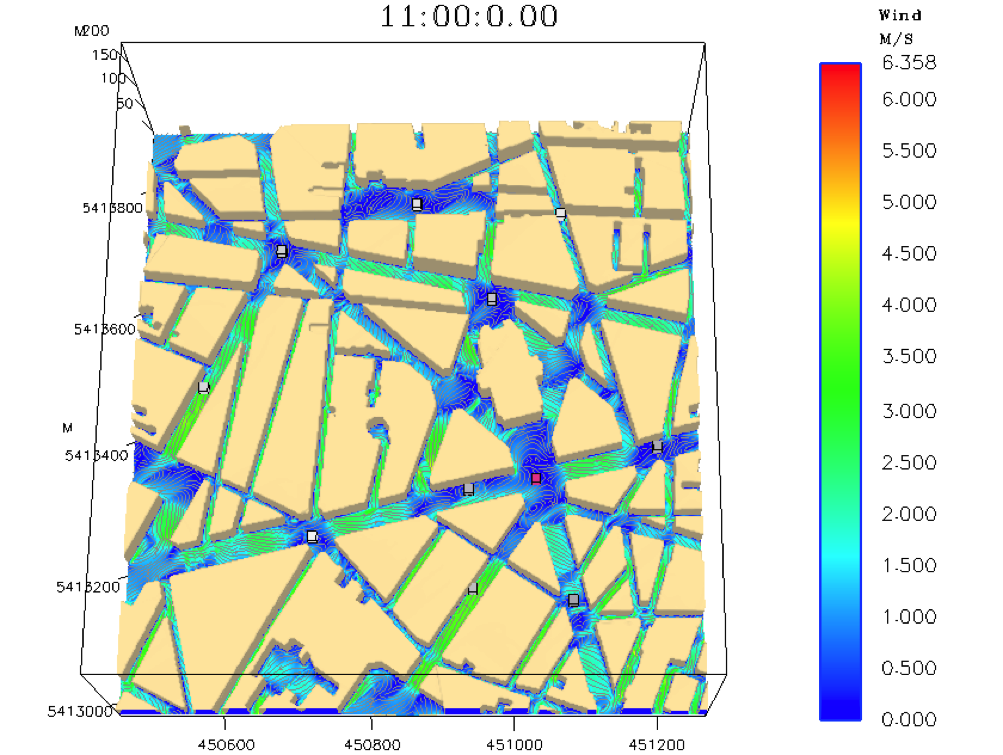
\includegraphics[width=1\textwidth]{opera_vent_11_00.png}
		\caption{}
		\label{opera_vent_11_00}
	\end{subfigure}%         	
	\begin{subfigure}[t]{0.5\textwidth}
		\centering
		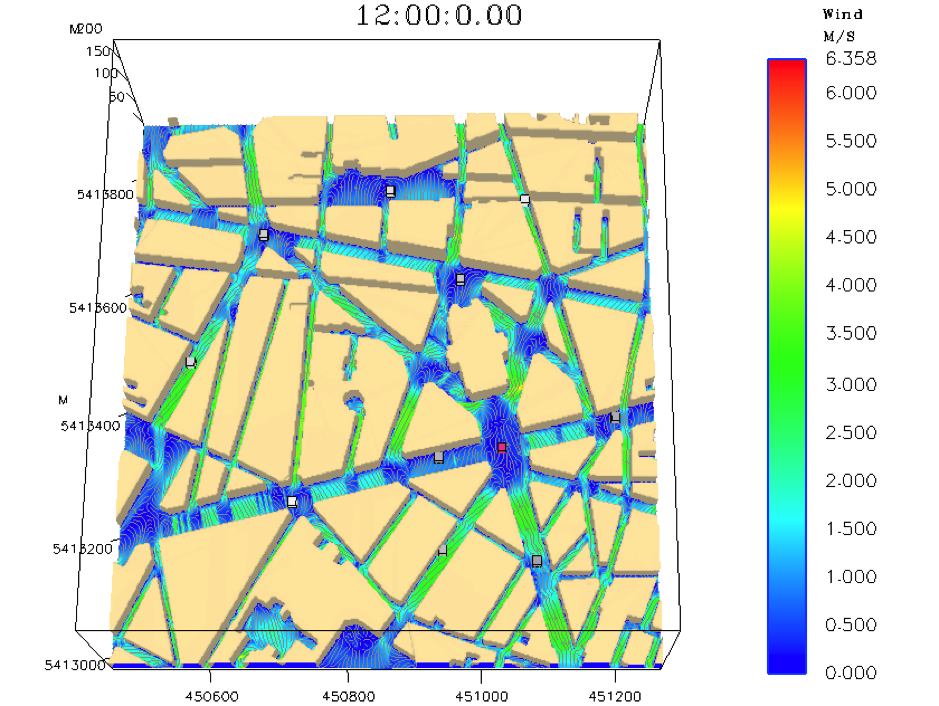
\includegraphics[width=1\textwidth]{opera_vent_12_00.png}
		\caption{}
		\label{opera_vent_12_00}
	\end{subfigure}
	\begin{subfigure}[t]{0.5\textwidth}
		\centering
		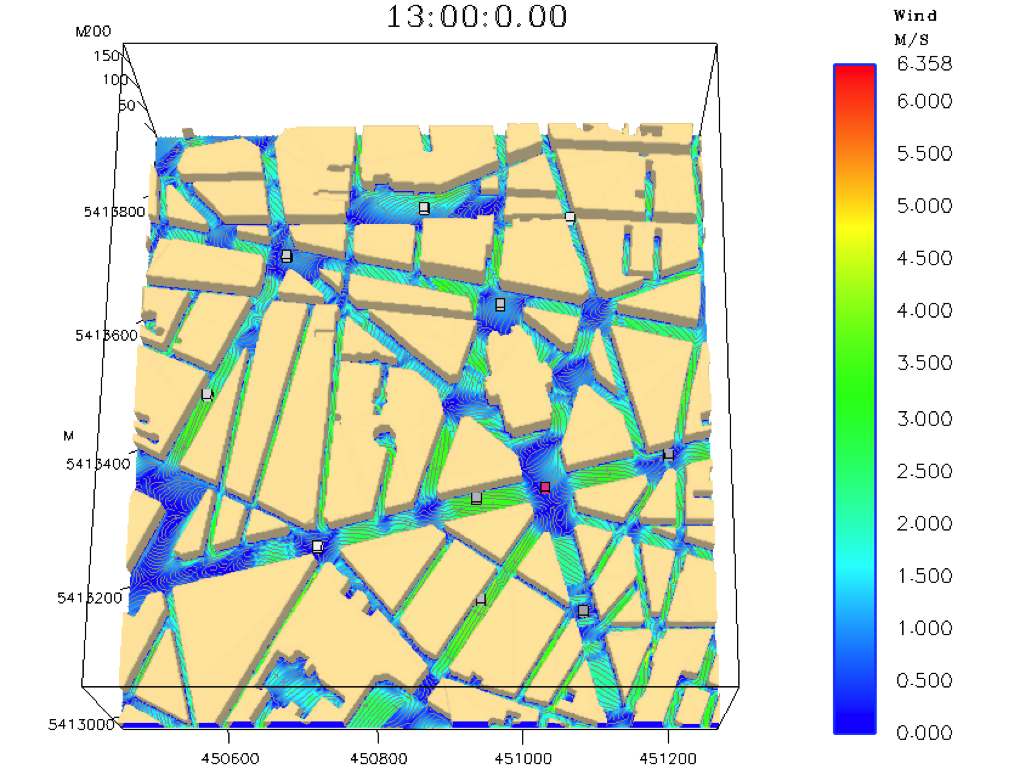
\includegraphics[width=1\textwidth]{opera_vent_13_00.png}
		\caption{}
		\label{opera_vent_13_00}
	\end{subfigure}%
	\caption{Champs de vent à \SI{2}{\meter} du sol produits par SWIFT aux trois échéances météorologiques considérées}
	\label{fig_opera_vent}
	
\end{figure}



\subsubsection{Capteurs, source et simulation des observations}
Le domaine contient un réseau de 10 capteurs, qui sont placés aux centres de diverses intersections de rues, ainsi que sur des places publiques. Ils sont situés à lune hauteur de 2m, et délivrent des valeurs de concentrations moyennées sur des plages de 5 minutes entre 11h35 et 13h.

La source est également située à 2m du sol, positionnée au niveau d'une grande intersection, et émet un rejet bref d'une durée de 10 minutes entre 12h10 et 12h20, avec un débit constant de $10^4$ unités/s. Ces caractéristiques se rapprochent de celles d'un rejet d'origine malveillante, par exemple suite à l'explosion d'une "bombe sale". 

On suit le même raisonnement que pour le cas-test Beaune et on simule le vecteur d'observations à partir d'une matrice source-récepteur \textit{backward} afin d'obtenir les mesures simulées de la figure \ref{fig_opera_obs}. Les dimensions de cette source sont celles d'une maille du domaine, à savoir un volume de 2m $\times$ 2m $\times$ 2m.

\begin{figure}[h!]
	\centering
	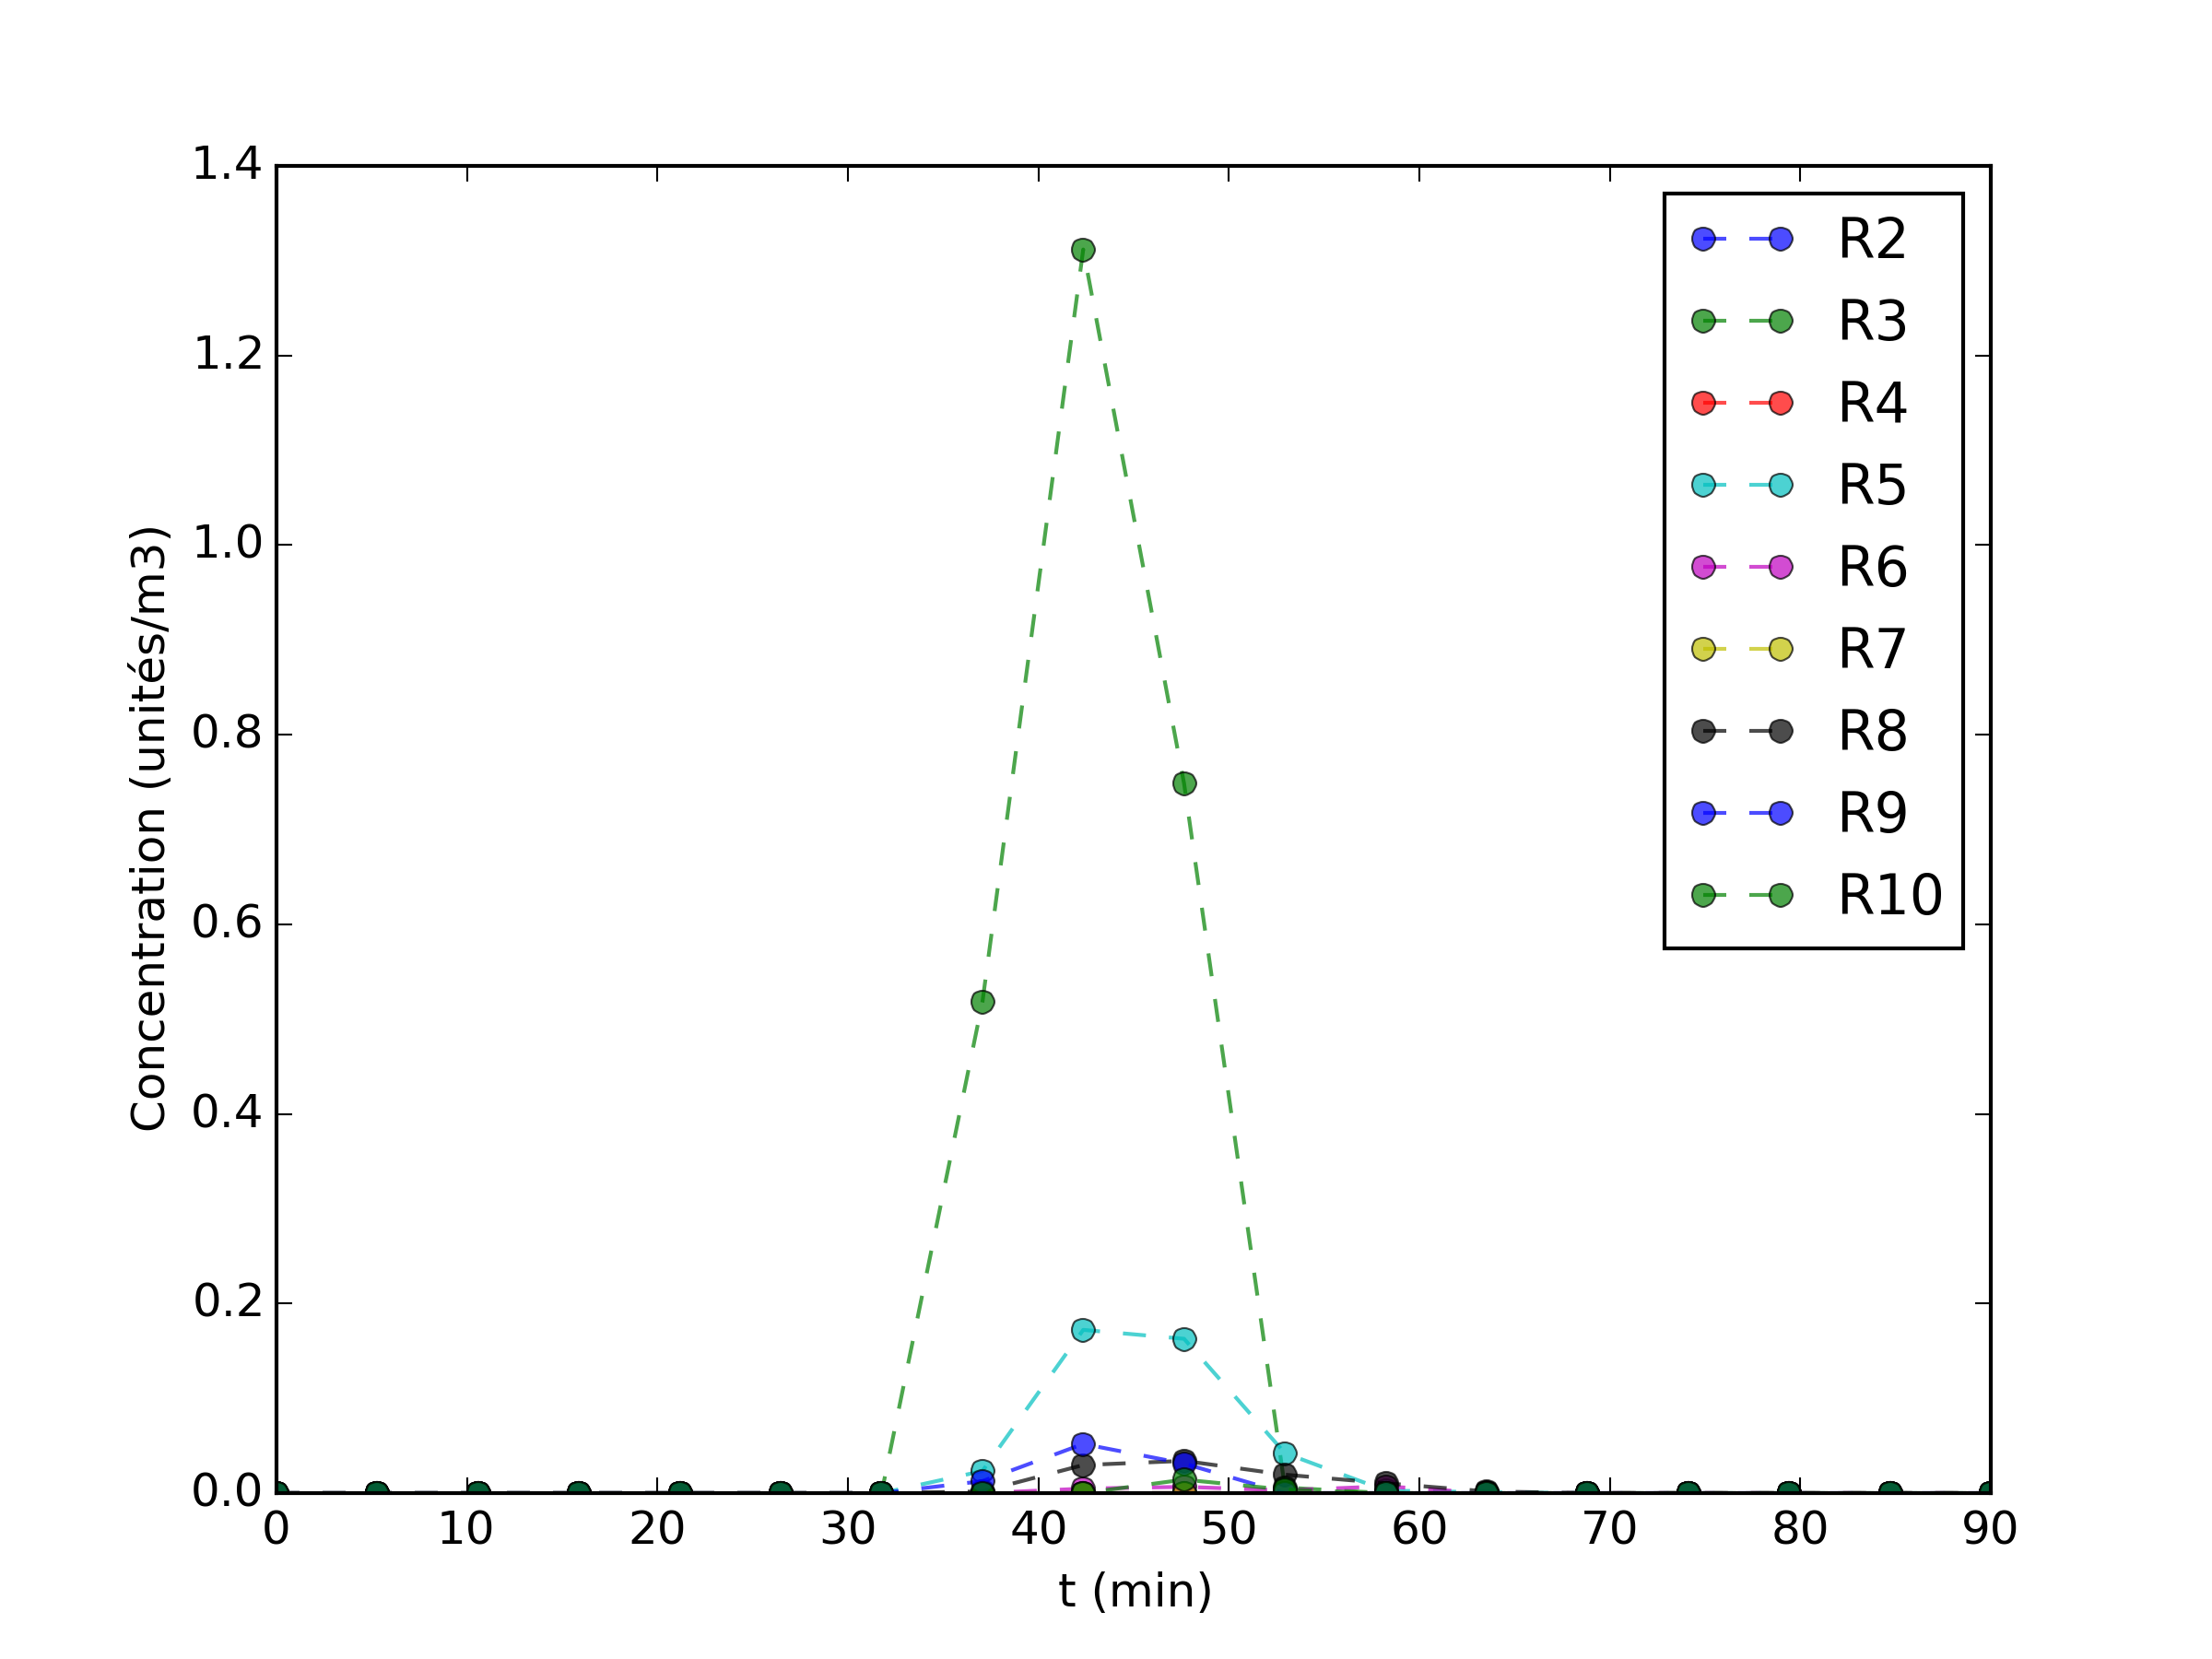
\includegraphics[width=0.8\textwidth]{concentrations_opera.png}
	\caption{Cas-test Opéra: concentrations mesurées aux capteurs}
	\label{fig_opera_obs}
\end{figure}

Etant donné la taille réduite du domaine ainsi que les conditions météorologiques instationnaires auquel le cas-test est confronté, on observe que malgré un nombre total de capteurs inférieur à celui du cas-test Beaune, la proportion de récepteurs mesurant une concentration non-nulle est ici plus élevée.


\subsection{Initialisation optimisée de la loi de proposition}

Dans une situation complexe comme celle du cas Opéra, il peut se révéler utile d'initialiser la loi de proposition pour l'AMIS de façon plus judicieuse qu'une simple hypothèse de répartition uniforme des particules sur le domaine. Une initialisation optimisée permet en effet d'explorer des zones potentiellement intéressantes plus rapidement, augmentant l'efficacité de l'algorithme d'estimation. \\

Comme dans notre cas on a choisi une loi de proposition de type mixture de $D$ gaussiennes $\varphi_1, \dots, \varphi_D$, on va chercher à estimer les moyennes $\left(\VecMu_d\right)_{1:d}$ et les matrices de covariance $\left(\MatSigma_d\right)_{1:d}$ de chacune de ces composantes, ainsi que leurs facteurs d'influence $\left(\alpha_d\right)_{1:d}$. 

Pour cela, in utilise les résultats issus d'un \textit{run} de rétro-propagation: suivant un modèle de dispersion dual tel que RetroSPRAY, on construit une série de cartes des concentrations conjuguées sur tout le domaine, en transformant les capteurs en rétro-sources et en utilisant les concentrations mesurées comme valeurs de rétro-émission. Une fois ces cartes créées, elles sont vues comme des ébauches des densités de probabilité sur la position de la source pour différents temps d'émission. L'objectif est alors de caler les paramètres $\left(\alpha_d, \VecMu_d,\MatSigma_d \right)_{1:D}$ sur ces densités.\\

On part de l'instant d'observation $t_0$ qui est celui où la concentration la plus élevée a été observée. On définit ensuite un instant $t_{RP}$ qui correspond à l'instant final de la rétro-propagation, avec $t_{RP} < t_0$.  

\subsection{Résultats}

